% Review examples adapted from the Grade 10 Term 1 C1--C7 and C8--C9
% solution keys and the separate Interactive Decision Webpage activity.
\makeatletter
\def\input@path{{../../../preamble/}{book2026-2027/preamble/}}
\makeatother
\input{preamble_G10_T1_C1C2C3}
\input{graphs/highlights}

\geometry{letterpaper,margin=0.72in}
\linespread{1.04}
\setlength{\parskip}{3pt}
\setlist[enumerate]{leftmargin=*,nosep}
\setlist[itemize]{leftmargin=*,nosep}
% Keep the standard heading anchors while tightening the review layout.
\makeatletter
\renewcommand{\section}{\@startsection{section}{1}{\z@}{-13pt}{5pt}{\normalfont\Large\bfseries}}
\renewcommand{\subsection}{\@startsection{subsection}{2}{\z@}{-11pt}{5pt}{\normalfont\large\bfseries}}
\makeatother
\setcounter{secnumdepth}{1}
\hypersetup{pdftitle={Grade 10 Global Economics \textemdash{} Term 1 Review Outline},
  linkcolor=black,urlcolor=black}

\newcommand{\Cue}{\textbf{When to use it.}\enspace}
\newcommand{\Example}[1]{\textbf{#1}\par}
\newcommand{\Decision}{\textbf{Decision.}\enspace}
\newcommand{\SourceValue}[1]{\HighlightStroke{black!25}{#1}}
\newcommand{\Deciding}[1]{\ensuremath{\boldsymbol{#1}}}
\newcommand{\ReviewLink}[1]{\hyperref[crit:#1]{\underline{\textbf{C#1}}}}
\newcommand{\BackToMap}{\par\noindent\hfill\hyperref[sec:summary]{\small\underline{Back to the summary}}\par}

% Compact versions of the filtering tree styles in the C8--C9 key.
\tikzset{
  cNine survivor/.style={draw,align=center,font=\small,text width=29mm,minimum height=6mm},
  cNine selected/.style={cNine survivor,very thick,fill=black!8},
  cNine eliminated/.style={align=left,font=\small,anchor=west},
  cNine keep/.style={-{Stealth},thick},
  cNine discard/.style={-{Stealth},dashed}
}

\begin{document}

{\centering
  {\LARGE\bfseries Grade 10 Global Economics\\[2pt]
  \textemdash{} Term 1 Review Outline\par}
  \smallskip 2026--2027\par
}

\section{Introduction}
First, identify what the decision maker can choose and what the world will reveal later. Next, organize the possible outcomes in a payoff table. Once the payoffs are clear, compare decisions under uncertainty, test how a recommendation changes, and apply criteria in sequence when the problem calls for several rounds of filtering.

\textbf{Review routine.} Identify the choice the decision maker controls. Organize outcomes by alternative and state, with a payoff measure and unit. Check the available probabilities and constraints. Apply the appropriate rule, show the values you compared, and justify the recommendation in context. Name all tied alternatives when applicable.

Scan the summary to recognize the task and find the method. Follow a criterion link to check your setup, intermediate calculations, and conclusion against a worked example.

\section{Summarized Outline}\label{sec:summary}
{\small
\begin{tabularx}{\linewidth}{@{}l L L L@{}}
\toprule
& \textbf{Cue in the question} & \textbf{Method} & \textbf{Write or draw}\\
\midrule
\ReviewLink{1} & Describe the decision. & Sort choices and states. & Who chooses, when, and what each payoff measures.\\
\ReviewLink{2} & Build a contribution table. & Add rates, scale, add fixed sum. & Formula, substitution, table.\\
\ReviewLink{3} & Build a profit table. & Revenue less both costs. & Revenue, costs, profit by cell.\\
\ReviewLink{4} & Optimistic or conservative? & Compare row maxima or minima. & Row statistics and winners.\\
\ReviewLink{5} & Limit missed profit. & Column bests, then row regrets. & Benchmarks, table, lowest max.\\
\ReviewLink{6} & Use state probabilities. & Find the weighted sum per row. & Probability check, terms, EMV.\\
\ReviewLink{7} & When does the choice change? & Find feasible bounds and EMV tie. & Equations, graph, intervals.\\
\ReviewLink{8} & Compare rules or change a payoff. & Update, screen, and rank. & Winners, values, tie or threshold.\\
\ReviewLink{9} & Filter options in stages. & Rank the survivors at each step. & Filtering table and tree.\\
\ReviewLink{10} & Justify a rule in context. & Match information and priorities. & Rationale and webpage checks.\\
\bottomrule
\end{tabularx}

\medskip
\textbf{Four rules for payoffs where more is better}
\par\smallskip
\begin{tabularx}{\linewidth}{@{}l c L l L L@{}}
\toprule
\textbf{Rule} & \textbf{Prob.?} & \textbf{Statistic} & \textbf{Choose} & \textbf{Priority} & \textbf{Limitation}\\
\midrule
Maximax & No & Row maximum & Highest & Greatest upside & Ignores downside.\\
Maximin & No & Row minimum & Highest & Best worst case & Can pass up large gains.\\
Minimax Regret & No & Row maximum regret & Lowest & Least worst missed profit & Depends on the comparison set.\\
EMV/Bayes & Yes & Row weighted sum & Highest & Highest expected payoff & Depends on probability estimates.\\
\bottomrule
\end{tabularx}

\medskip
\noindent
\begin{minipage}{0.24\linewidth}
\centering
\begin{tikzpicture}[>=Stealth]
  \draw (0,0) grid[xstep=.55,ystep=.37] (1.65,.74);
  \draw[->,thick] (.06,.55) -- (1.59,.55);
  \draw[->,thick,dashed] (.82,.78) -- (.82,-.13);
\end{tikzpicture}
\end{minipage}\hfill
\begin{minipage}{0.73\linewidth}
\textbf{Across a row} (solid) gives one alternative's maximum, minimum, EMV, or maximum regret.
\textbf{Down a state column} (dashed) gives the best payoff to use as that state's regret benchmark.
\end{minipage}
}

\clearpage
\section{Step-by-Step Outline}
In the examples, a \SourceValue{shaded value} marks the payoff being traced. \textbf{Bold deciding values} mark the statistic used to justify a recommendation. Always carry the original monetary unit through the calculation.

\subsection{C1 \textemdash{} Identify the decision elements}\label{crit:1}
\Cue The question asks you to characterize a choice under uncertainty.
\begin{enumerate}
  \item Name the decision maker, the economic purpose, and the alternatives they control.
  \item List the states of nature in order and say when the actual state is revealed.
  \item Explain how the state changes the outcome and name the payoff measure.
\end{enumerate}
\textbf{Craft Workshop.} The studio chooses a workshop to earn a net contribution.
\DecisionElementsTable
  {Pottery workshop; Weaving workshop}
  {Strong tourist demand; Weak tourist demand}
  {The studio cannot control tourist demand. It learns the demand state after choosing.}
  {Demand changes attendance and the extra contribution per participant. Each payoff is the total net contribution in USD for one workshop and one demand state.}
For Pottery under strong demand, \(12+6=18\) USD per participant before sponsorship. The studio controls the workshop choice. Demand determines which of that workshop's payoffs it earns.

\subsection{C2 \textemdash{} Build a payoff table from contributions}\label{crit:2}
\Cue The givens include per-participant contributions, attendance, and a fixed amount.
\begin{enumerate}
  \item Put alternatives \(A_i\) in rows and states \(S_j\) in columns.
  \item Add the workshop rate \(v_i\) and the demand addition \(d_j\), both in USD per participant.
  \item For each cell, multiply by attendance \(q_{ij}\) and add sponsorship \(f_i\) once,
        \(P_{ay}(A_i,S_j)=q_{ij}(v_i+d_j)+f_i\).
\end{enumerate}
\textbf{Craft Workshop, continued.} Pottery and Weaving contribute \(12,15\) USD per participant and receive sponsorships of \(80,50\) USD, respectively. Strong and weak demand add \(6,2\) USD per participant.
\CalculationPair{Net contribution (USD)}{
  \begin{tabular}{@{}lcc@{}}
  \toprule & Strong (\(S_1\)) & Weak (\(S_2\))\\\midrule
  \(A_1\) & \SymbolicCell{q_{11}(v_1+d_1)+f_1}{P_{ay}(A_1,S_1)}
          & \SymbolicCell{q_{12}(v_1+d_2)+f_1}{P_{ay}(A_1,S_2)}\\
  \(A_2\) & \SymbolicCell{q_{21}(v_2+d_1)+f_2}{P_{ay}(A_2,S_1)}
          & \SymbolicCell{q_{22}(v_2+d_2)+f_2}{P_{ay}(A_2,S_2)}\\
  \bottomrule
  \end{tabular}
}{
  \begin{tabular}{@{}lcc@{}}
  \toprule & Strong (\(S_1\)) & Weak (\(S_2\))\\\midrule
  \(A_1\) & \CalcResult{30(12+6)+80}{\SourceValue{620}} & \CalcResult{18(12+2)+80}{332}\\
  \(A_2\) & \CalcResult{24(15+6)+50}{554} & \CalcResult{16(15+2)+50}{322}\\
  \bottomrule
  \end{tabular}
}
\FinalPayoffTable{net contribution in USD}{Strong (\(S_1\)) & Weak (\(S_2\))}{
  Pottery workshop (\(A_1\)) & \(\SourceValue{620}\) & 332\\
  Weaving workshop (\(A_2\)) & 554 & 322\\
}
\Decision The Pottery workshop earns the higher contribution under both strong and weak demand.
\BackToMap

\clearpage
\subsection{C3 \textemdash{} Build a profit table from revenue and costs}\label{crit:3}
\Cue You have sales quantities, revenue per sale, variable costs, and fixed costs.
\begin{enumerate}
  \item Multiply places sold \(q_{ij}\) by base revenue \(b_i\) plus the per-sale surcharge \(s_j\).
  \item Multiply \(q_{ij}\) by the variable cost per place \(c_i\).
  \item Subtract total variable cost and the fixed seasonal cost \(F_j\) once. Enter the profit in its row and column.
\end{enumerate}
\Example{Guided Cycling Tours}
Town and Countryside have base revenues \(32,45\) and variable costs \(18,26\), in USD per place.
Strong and weak demand add \(8,3\) USD per place and incur fixed seasonal costs of \(500,650\) USD.

\CalculationPair{Trace Town under strong demand (USD)}{
  \begin{tabular}{@{}ll@{}}
  \toprule \textbf{Component} & \textbf{Expression}\\\midrule
  Revenue & \(R_{11}=q_{11}(b_1+s_1)\)\\
  Variable cost & \(VC_{11}=q_{11}c_1\)\\
  Profit & \(P(A_1,S_1)=R_{11}-VC_{11}-F_1\)\\
  \bottomrule
  \end{tabular}
}{
  \begin{tabular}{@{}l@{}}
  \toprule \textbf{Substitution for 90 places}\\\midrule
  \(90(32+8)=3600\)\\
  \(90(18)=1620\)\\
  \(3600-1620-500=\SourceValue{1480}\)\\
  \bottomrule
  \end{tabular}
}
{\centering\small
\begin{tabular}{@{}llrrrrr@{}}
\toprule
Route & Demand & Places & Revenue & Variable cost & Fixed cost & Profit (USD)\\
\midrule
Town (\(A_1\)) & Strong (\(S_1\)) & 90 & 3600 & 1620 & 500 & \(\SourceValue{1480}\)\\
               & Weak (\(S_2\)) & 60 & 2100 & 1080 & 650 & 370\\
Countryside (\(A_2\)) & Strong (\(S_1\)) & 70 & 3710 & 1820 & 500 & 1390\\
                      & Weak (\(S_2\)) & 40 & 1920 & 1040 & 650 & 230\\
\bottomrule
\end{tabular}\par}
\FinalPayoffTable{seasonal profit in USD}{Strong (\(S_1\)) & Weak (\(S_2\))}{
  Town route (\(A_1\)) & \(\SourceValue{1480}\) & 370\\
  Countryside route (\(A_2\)) & 1390 & 230\\
}
\Decision The town route has higher seasonal profit in both demand states.

\subsection{C4 \textemdash{} Compare Maximax and Maximin}\label{crit:4}
\Cue The question asks for an optimistic choice or the best protection against a poor outcome.
\begin{enumerate}
  \item For Maximax, find the maximum payoff \(M_i\) in each row and choose the highest \(M_i\).
  \item For Maximin, find the minimum payoff \(m_i\) in each row and choose the highest \(m_i\).
\end{enumerate}
\Example{Sportswear Stock}
A retailer chooses a stock plan with no demand probabilities. Profits are in thousand USD.\par
{\centering\small
\begin{tabular}{@{}lrrrrr@{}}
\toprule
Alternative & High & Medium & Low & Row max \(M_i\) & Row min \(m_i\)\\
\midrule
Bulk order (\(A_1\)) & 120 & 48 & \(-30\) & \(\Deciding{120}\) & \(-30\)\\
Regular order (\(A_2\)) & 84 & 57 & 16 & 84 & 16\\
Small order (\(A_3\)) & 55 & 43 & \(\SourceValue{29}\) & 55 & \(\Deciding{29}\)\\
Pre-orders only (\(A_4\)) & 24 & 24 & 24 & 24 & 24\\
\bottomrule
\end{tabular}\par}
\Decision Maximax selects \textbf{Bulk order}, with an upside of 120 and a possible loss of 30.
Maximin selects \textbf{Small order}. Its minimum, \(\min\{55,43,\SourceValue{29}\}=\Deciding{29}\), gives the best protection, with an upside of 55.
\BackToMap

\clearpage
\subsection{C5 \textemdash{} Minimize maximum regret}\label{crit:5}
\Cue The decision maker wants to limit the largest profit they could miss.
\begin{enumerate}
  \item Compare down each state column to find its best payoff \(b_j\).
  \item Subtract each payoff from its column benchmark, \(r_{ij}=b_j-P(A_i,S_j)\).
  \item Find the largest regret in each row and choose the smallest of those row maxima.
\end{enumerate}
\Example{Flower Stall}
A florist chooses a purchasing plan before holiday demand is known. Regret is the extra profit the florist could have earned by choosing the best plan for the state that occurred. Both tables use thousand USD.

\noindent
\begin{minipage}[t]{0.51\linewidth}
\centering\small
\textbf{Payoffs}\par\smallskip
\setlength{\tabcolsep}{3.5pt}
\begin{tabular}{@{}lrrr@{}}
\toprule
Alternative & High & Medium & Low\\
\midrule
Large purchase (\(A_1\)) & 78 & 32 & \(-12\)\\
Medium purchase (\(A_2\)) & \(\SourceValue{60}\) & 48 & 18\\
Small purchase (\(A_3\)) & 40 & 38 & 30\\
\midrule
State best \(b_j\) & 78 & 48 & 30\\
\bottomrule
\end{tabular}
\end{minipage}\hfill
\begin{minipage}[t]{0.46\linewidth}
\centering\small
\textbf{Regrets}\par\smallskip
\setlength{\tabcolsep}{3.5pt}
\begin{tabular}{@{}lrrrr@{}}
\toprule
Plan & High & Medium & Low & Row max\\
\midrule
\(A_1\) & 0 & 16 & 42 & 42\\
\(A_2\) & 18 & 0 & 12 & \(\Deciding{18}\)\\
\(A_3\) & 38 & 10 & 0 & 38\\
\bottomrule
\end{tabular}
\end{minipage}

For \(A_2\), the regrets are \(78-\SourceValue{60}=18\), \(48-48=0\), and \(30-18=12\).
For \(A_1\) under low demand, subtracting a negative payoff gives \(30-(-12)=42\).
The smallest row maximum is \(\min\{42,18,38\}=\Deciding{18}\).
\Decision Choose \textbf{Medium purchase} (\(A_2\)). Its largest possible missed profit is 18 thousand USD.

\subsection{C6 \textemdash{} Calculate EMV and apply Bayes}\label{crit:6}
\Cue The question supplies state probabilities and asks for the highest expected payoff.
\begin{enumerate}
  \item Check that each \(P(S_j)\) is in \([0,1]\) and that the probabilities sum to one.
  \item For each row, multiply each payoff by its matching column probability and add the products, \(\mathrm{EMV}(A_i)=\sum_j P(S_j)P(A_i,S_j)\).
  \item Compare the totals and report the highest expected payoff in the original units.
\end{enumerate}
\Example{Fruit Packing}
A cooperative chooses a packing plan before export demand is known. Payoffs and EMVs are in thousand USD.
\begin{center}\small
\begin{tabular}{@{}lrrr@{}}
\toprule
Alternative & Strong & Steady & Weak\\
\(P(S_j)\) & 0.40 & 0.35 & 0.25\\
\midrule
Premium packs (\(A_1\)) & 90 & 44 & \(-12\)\\
Mixed packs (\(A_2\)) & \(\SourceValue{68}\) & 58 & 24\\
Basic packs (\(A_3\)) & 46 & 48 & 38\\
\bottomrule
\end{tabular}
\end{center}
Each probability is in \([0,1]\), and \(0.40+0.35+0.25=1\).
\begin{align*}
\mathrm{EMV}(A_1)&=0.40(90)+0.35(44)+0.25(-12)=36+15.40-3=48.40,\\
\mathrm{EMV}(A_2)&=0.40(\SourceValue{68})+0.35(58)+0.25(24)=27.20+20.30+6=\Deciding{53.50},\\
\mathrm{EMV}(A_3)&=0.40(46)+0.35(48)+0.25(38)=18.40+16.80+9.50=44.70.
\end{align*}
\Decision Choose \textbf{Mixed packs} (\(A_2\)). Under the stated probabilities, expected profit is 53.50 thousand USD (USD 53,500). The profit actually earned depends on which state occurs.
\BackToMap

\clearpage
\subsection{C7 \textemdash{} Find where the EMV recommendation changes}\label{crit:7}
\Cue A state probability depends on \(p\), and the question asks which option wins as \(p\) changes.
\begin{enumerate}
  \item Use the sum-to-one condition to express the missing probability in terms of \(p\).
  \item Require every probability to lie in \([0,1]\). Intersect the resulting bounds.
  \item Write the competing EMVs as functions of \(p\). Set them equal and check the tie is feasible.
  \item Compare on each side and at the feasible endpoints. Report the winner by interval, including the tie and any infeasible values.
\end{enumerate}
\Example{Online Course Launch}
A training business chooses a launch plan before enrolment is known. Profits are in thousand USD.
\begin{center}\small
\begin{tabular}{@{}lrrr@{}}
\toprule
Alternative & High (\(S_1\)) & Moderate (\(S_2\)) & Low (\(S_3\))\\
\(P(S_j)\) & \(p\) & \(p/2\) & \(1-3p/2\)\\
\midrule
Full (\(A_1\)) & 100 & 36 & \(-8\)\\
Pilot (\(A_2\)) & 52 & 48 & 28\\
\bottomrule
\end{tabular}
\end{center}
From \(p+p/2+P(S_3)=1\), we get \(P(S_3)=1-3p/2\).
The three probability checks give \(0\le p\le1\), \(0\le p\le2\), and \(0\le p\le2/3\), respectively.
The feasible range is their intersection, \(\boxed{0\le p\le2/3}\).
\begin{align*}
E_1(p)&=100p+36(p/2)-8(1-3p/2)=130p-8,\\
E_2(p)&=52p+48(p/2)+28(1-3p/2)=28+34p.
\end{align*}
The tie solves \(130p-8=28+34p\), so \(96p=36\) and \(p=3/8\) is feasible. Both EMVs equal \(40.75\) thousand USD there.
The difference \(E_1-E_2=96p-36\) is negative below the tie and positive above it.
At \(p=0\), \((E_1,E_2)=(-8,28)\). At \(p=2/3\), \((E_1,E_2)=(236/3,152/3)\).

\medskip
\noindent
\begin{minipage}[c]{0.40\linewidth}
\raggedright
\Decision Choose the launch with the higher expected profit at your feasible value of \(p\).
\begin{center}
\small
\begin{tabular}{@{}ll@{}}
\toprule
\(p\) & Recommendation\\
\midrule
\(0\le p<3/8\) & Pilot (\(A_2\))\\
\(p=3/8\) & Both tied\\
\(3/8<p\le2/3\) & Full (\(A_1\))\\
\bottomrule
\end{tabular}
\end{center}
For \(2/3<p\le1\), the low-enrolment probability is negative, so these inputs are infeasible.
\end{minipage}\hfill
\begin{minipage}[c]{0.57\linewidth}
\centering
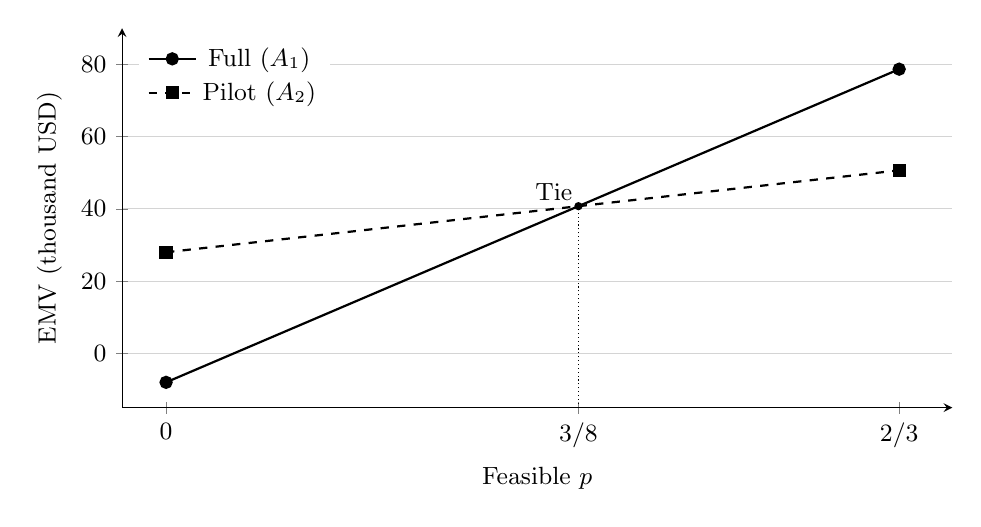
\begin{tikzpicture}
\begin{axis}[
  width=\linewidth,height=6.4cm,
  xmin=-.04,xmax=.715,ymin=-15,ymax=90,
  axis lines=left,
  xlabel={Feasible \(p\)},ylabel={EMV (thousand USD)},
  xtick={0,0.375,0.6666667},xticklabels={\(0\),\(3/8\),\(2/3\)},
  ytick={0,20,40,60,80},
  tick label style={font=\small},label style={font=\small},
  ymajorgrids,grid style={black!17},
  legend style={at={(.02,.98)},anchor=north west,font=\small,draw=none,fill=white}
]
\addplot[black,thick,mark=*,mark options={solid},samples=2,domain=0:2/3] {130*x-8};
\addlegendentry{Full (\(A_1\))}
\addplot[black,thick,dashed,mark=square*,mark options={solid},samples=2,domain=0:2/3] {28+34*x};
\addlegendentry{Pilot (\(A_2\))}
\draw[thin,densely dotted] (axis cs:.375,-15) -- (axis cs:.375,40.75);
\fill (axis cs:.375,40.75) circle[radius=1.5pt];
\node[font=\small,anchor=south east,inner sep=2pt] at (axis cs:.375,40.75) {Tie};
\end{axis}
\end{tikzpicture}
\end{minipage}
\BackToMap

\clearpage
\subsection{C8 \textemdash{} Compare rules and test payoff changes}\label{crit:8}
\Cue The question compares methods or asks when a revised payoff changes the recommendation.
\begin{enumerate}
  \item Use the same starting payoff table for all four rules. Record each recommendation and its deciding value.
  \item Change only the specified payoffs. Apply the stated eligibility rule before ranking the remaining alternatives.
  \item Recalculate the relevant statistics on the eligible set. For regret, recompute the state benchmarks on that set.
  \item Use a strict inequality for a sole winner. Check the tie and the first permitted integer beyond it.
\end{enumerate}
\Example{Repair Workshop Plans}
A bicycle repair workshop chooses its capacity. Profits and deciding values are in thousand USD.
\begin{center}\small
\setlength{\tabcolsep}{4.5pt}
\begin{tabular}{@{}lrrr@{\hspace{1.2em}}rrrr@{}}
\toprule
 & \multicolumn{3}{c}{Payoffs} & \multicolumn{4}{c}{Decision statistics}\\
\cmidrule(lr){2-4}\cmidrule(l){5-8}
Alternative & High & Normal & Low & Max & Min & Max regret & EMV\\
\(P(S_j)\) & 0.2 & 0.6 & 0.2 & & & & \\
\midrule
Large (\(A_1\)) & 120 & 25 & \(-20\) & \(\Deciding{120}\) & \(-20\) & 55 & 35\\
Flexible (\(A_2\)) & 85 & 65 & \(-10\) & 85 & \(-10\) & \(\Deciding{45}\) & 54\\
Basic (\(A_3\)) & 50 & 45 & 35 & 50 & \(\Deciding{35}\) & 70 & 44\\
Partner (\(A_4\)) & 70 & 75 & 20 & 75 & 20 & 50 & \(\Deciding{63}\)\\
\bottomrule
\end{tabular}
\end{center}
The state bests are \((120,75,35)\), so \(A_2\)'s maximum regret is
\(\max\{120-85,75-65,35-(-10)\}=45\).
The Partner plan's EMV is \(0.2(70)+0.6(75)+0.2(20)=14+45+4=63\).

\Decision Maximax chooses \textbf{Large} at 120. Maximin chooses \textbf{Basic} at 35.
Minimax Regret chooses \textbf{Flexible} at 45. EMV/Bayes chooses \textbf{Partner} at 63.

\textbf{Variant. Subsidy and Maximin.}
For integer \(0\le s\le50\), replace the Low payoffs for \(A_1,A_2\) with \(-20+s,-10+s\). All payoffs must be nonnegative. \(A_1\) becomes eligible at \(s=20\), \(A_2\) at \(s=10\), and \(A_3,A_4\) are always eligible.
The row minima in order are \(\min\{25,-20+s\},-10+s,35,20\).
Only \(A_2\) can overtake \(A_3\), since \(A_1\)'s minimum is at most 25 and \(A_4\)'s is 20.
Flexible ties Basic at \(s=45\), since \(-10+45=35\). It wins uniquely when \(-10+s>35\). The first such integer is \(\Deciding{s=46}\), when its minimum profit is 36 thousand USD.

\Example{Community Market Stall}
Profits are in hundred USD. A sponsor replaces Compact's High payoff of \(48\) with an integer \(g\) in \([48,80]\). Both payoffs must be at least 20.
\begin{center}\small
\begin{tabular}{@{}lrrl@{}}
\toprule
Alternative & High & Low & Eligible for this range?\\
\midrule
Large (\(C_1\)) & 80 & 10 & No\\
Compact (\(C_2\)) & \(g\) & 32 & Yes\\
Standard (\(C_3\)) & 70 & 25 & Yes\\
Premium (\(C_4\)) & 90 & \(-5\) & No\\
\bottomrule
\end{tabular}
\end{center}
The original unrestricted benchmarks were \((90,32)\), and Standard won on maximum regret \(20\).
After screening, the benchmarks are \((\max\{g,70\},32)\).
Thus \(R(C_2)=\max\{70-g,0\}\) and \(R(C_3)=\max\{g-70,7\}\).
Up to \(g=70\), compare \(70-g\) with \(7\). At \(g=63\) both regrets equal 7. The first integer with \(70-g<7\) is \(\Deciding{g=64}\).
Compact then wins with regret 6 versus 7, and its high-attendance profit is USD 6,400.
\BackToMap

\clearpage
\subsection{C9 \textemdash{} Apply criteria in stages}\label{crit:9}
\Cue The question gives an ordered list of rules and tells you how many alternatives to keep.
\begin{enumerate}
  \item Start with all eligible alternatives. Apply the first rule and rank its deciding values in the correct direction.
  \item Keep the required alternatives. Record survivors, eliminations, and their values. If a tie crosses a cutoff, use the problem's tie rule or report the unresolved tie if none is given.
  \item At each later stage, compare only survivors. Use the supplied statistics when given. If the task calls for fresh regrets, find the benchmarks on the current comparison set.
  \item Draw solid arrows for survivors and dashed arrows for eliminations. Mark the final choice or report a final tie under the stated rules.
\end{enumerate}
\Example{Book Fair Stock}
The bookseller compares plans \(D_1\) through \(D_6\). All deciding values below are in hundred USD.

\medskip
\noindent
\begin{minipage}[c]{0.62\linewidth}
\small
\setlength{\tabcolsep}{3pt}
\begin{tabularx}{\linewidth}{@{}L L L@{}}
\toprule
Stage and rule & Survivors (value) & Eliminated (value)\\
\midrule
0. Start & \(D_1\) through \(D_6\) & \textemdash\\
1. EMV/Bayes, best 3 & \(D_1(65)\), \(D_2(65)\), \(D_3(65)\) & \(D_4(59)\), \(D_5(53)\), \(D_6(43)\)\\
2. Maximax, best 2 & \(D_1(100)\), \(D_2(90)\) & \(D_3(80)\)\\
3. Maximin, final & \(\Deciding{D_2(10)}\) & \(D_1(0)\)\\
\bottomrule
\end{tabularx}
\end{minipage}\hfill
\begin{minipage}[c]{0.36\linewidth}
\centering
\begin{tikzpicture}
  \node[cNine survivor] (s0) at (0,0) {All six \(D_i\)};
  \node[cNine survivor] (s1) at (0,-1.15) {\(D_1,D_2,D_3\)};
  \node[cNine survivor] (s2) at (0,-2.30) {\(D_1,D_2\)};
  \node[cNine selected] (s3) at (0,-3.45) {\textbf{Selected \(D_2\)}};
  \node[cNine eliminated] (e1) at (1.58,-.575) {Out \(D_4,D_5,D_6\)};
  \node[cNine eliminated] (e2) at (1.58,-1.725) {Out \(D_3\)};
  \node[cNine eliminated] (e3) at (1.58,-2.875) {Out \(D_1\)};
  \draw[cNine keep] (s0) -- coordinate[midway] (b1) node[left,font=\small] {1} (s1);
  \draw[cNine keep] (s1) -- coordinate[midway] (b2) node[left,font=\small] {2} (s2);
  \draw[cNine keep] (s2) -- coordinate[midway] (b3) node[left,font=\small] {3} (s3);
  \draw[cNine discard] (b1) -- (e1);
  \draw[cNine discard] (b2) -- (e2);
  \draw[cNine discard] (b3) -- (e3);
\end{tikzpicture}
\end{minipage}\par
\medskip
All three plans with EMV 65 fit into the three available places. Next \(100>90>80\) leaves \(D_1,D_2\).

\Decision The bookseller selects \textbf{\(D_2\)}. Of the two finalists, it has the higher worst-case profit, 10 hundred USD (USD 1,000).

\subsection{C10 \textemdash{} Justify a criterion in context}\label{crit:10}
\Cue The question asks which rule suits the decision maker and why.
\begin{enumerate}
  \item Check whether credible state probabilities are available.
  \item Identify the decision maker's priority and willingness to accept a poor outcome.
  \item Choose the rule that fits, show its deciding calculation, and explain what the result means for this decision.
\end{enumerate}
\Example{Sportswear Stock, with a cash constraint}
Suppose the retailer has no reliable demand probabilities and needs to protect cash in a weak season. The row minima from \ReviewLink{4} are \(-30,16,29,24\) thousand USD. Maximin fits that priority because it compares the worst outcomes. Since \(\max\{-30,16,29,24\}=\Deciding{29}\), the retailer should choose \textbf{Small order}, whose lowest listed profit is 29 thousand USD.

\textbf{Interactive Decision Webpage activity checklist.}
Use the same reasoning to interpret the webpage's recommendations. Check that users can do the following.
\begin{itemize}[label=\(\square\)]
  \item Add, edit, and remove alternatives and states. Edit payoffs and state probabilities.
  \item Compare all four rules with their values, recommendations, and any ties.
  \item Apply staged filtering and see each elimination and the final result in a flow diagram.
  \item Select at least two distinct preloaded scenarios, each with alternatives, states, payoffs, and probabilities, to test all four rules, filtering, and the diagram.
  \item See calculations and visuals update automatically. Check that the layout is clear and responsive, results agree, and invalid inputs are handled.
  \item Find a visible, accessible link to the AI development conversation.
\end{itemize}
\BackToMap

\end{document}



